\documentclass[a4paper,10pt]{scrartcl}

\usepackage{polski}
\usepackage[utf8]{inputenc}
\usepackage{graphicx}

\title{Laboratorium 2}
\author{Filip Malinowski}
\date{\today}

\pdfinfo{%
  /Title    (Laboratorium 2)
  /Author   (Filip Malinowski)
}

\begin{document}

\title{Sprawozdanie z laboratorium 2}
\author{Filip Malinowski}
\date{\today}

\maketitle

W zadaniu są dwa programy. Pierwszy generuje dane wejściowe.
Drugi jest odpowiedzialny za uruchamianie kolejno czterech
algorytm. Oba programy uruchamiane są przez Makefile.
Ilość danych wejściowych jest konfigurowana w kodzie źródłowym.
Program testujący algorytm składa się z klasy bazowej
Benchmark i klas pochodnych:
\begin{itemize}
 \item Mnozenie
 \item AlgorithmStos
 \item AlgorithmKolejka
 \item AlgorithmLista
\end{itemize}

Klasa Benchmark wyznacza odstęp czasowy za pomocą pomiaru czasu
przy użyciu biblioteki chrono. Następie tworzone są 4 pliki
wyjściowe, do których zapisywane są dane o szybkości wykonanych
algorytmów. Dane zapisywane są odpowiednio:
\begin{enumerate}
 \item mnożenie n elementów tablicy przez 2 - ret data1.txt
 \item wprowadzanie do stosu n elementów - ret data2.txt
 \item wprowadzanie do kolejki n elementów - ret data3.txt
 \item wprowadzanie do listy n elementów - ret data4.txt
\end{enumerate}

\begin{figure}
 \centering
  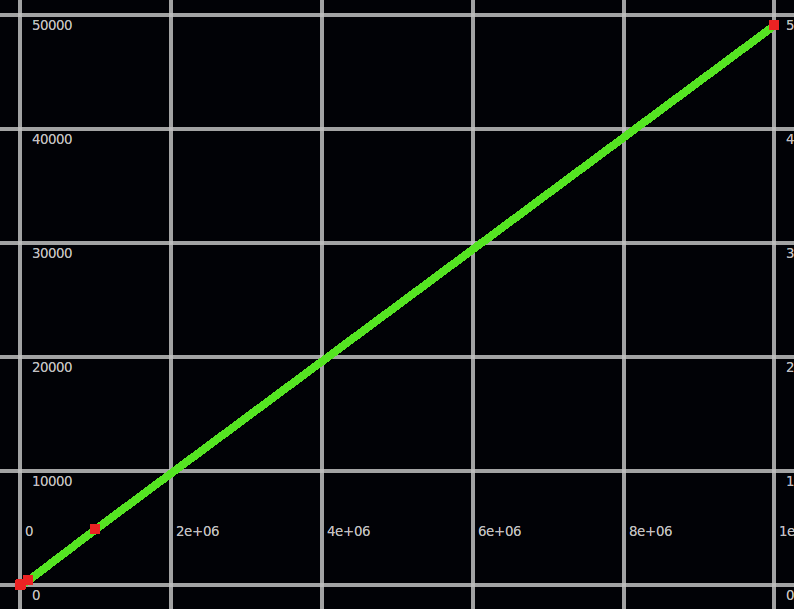
\includegraphics[scale=0.4]{ret_data1}
 \caption{Wykres dla mnożenia elementów tablicy przez 2}
\end{figure}

\begin{figure}
 \centering
  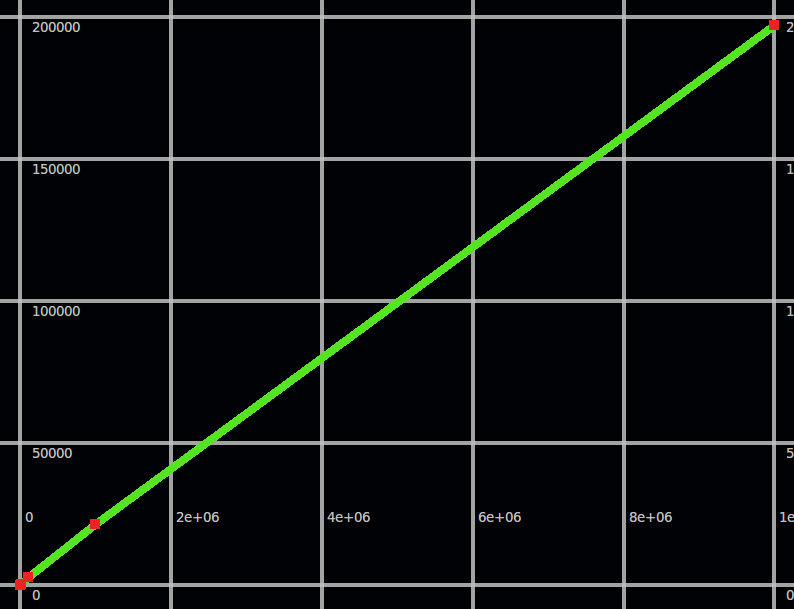
\includegraphics[scale=0.4]{ret_data2}
 \caption{Wykres dla wczytywania n elementów do stosu}
\end{figure}

\begin{figure}
 \centering
  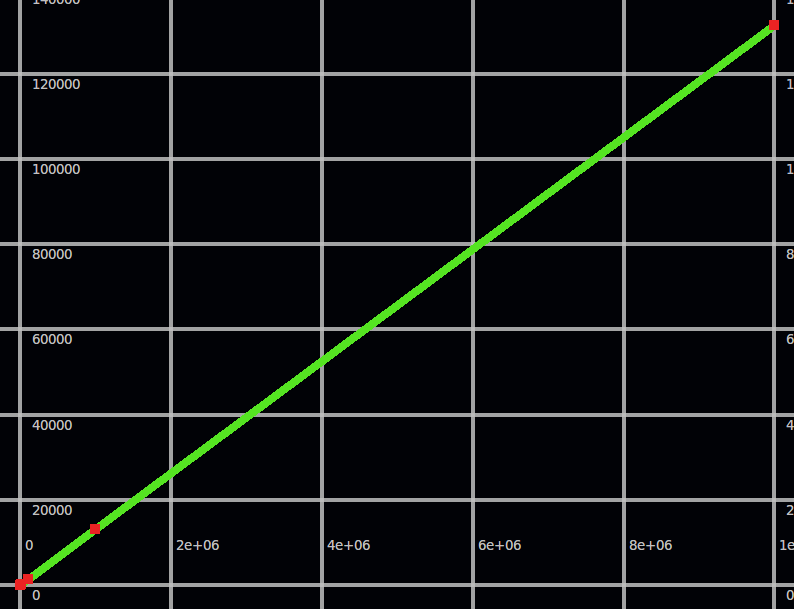
\includegraphics[scale=0.4]{ret_data3}
 \caption{Wykres dla wczytywania n elementów do kolejki}
\end{figure}

\begin{figure}
 \centering
  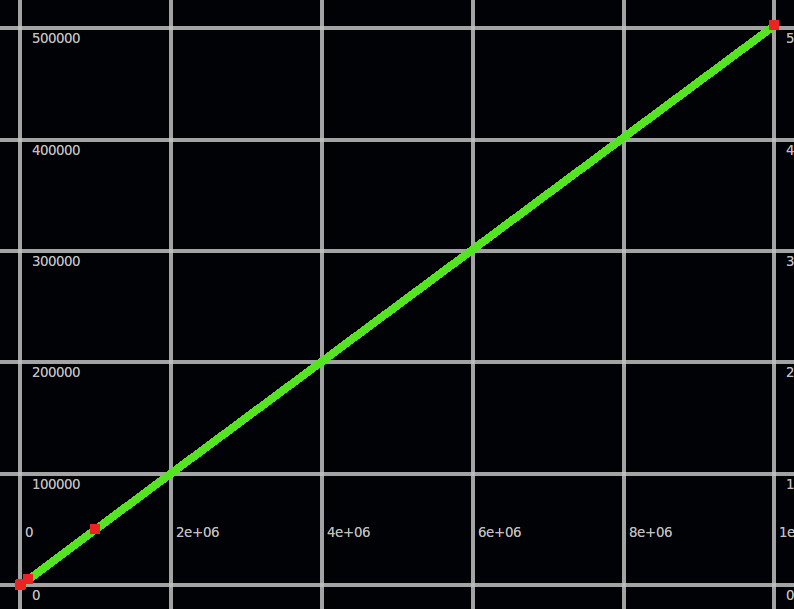
\includegraphics[scale=0.4]{ret_data4}
 \caption{Wykres dla wczytywania n elementów do listy}
\end{figure}

\end{document}
